\chapter{Alternation Rules}

\section{What are Alternation Rules?}

Alternation rules are extensions of the regular-expression language, and each alternation rule compiles into a
finite-state transducer.  As always, finite-state transducers encode regular relations, and the ``action'' of a rule,
which appears superficially to be algorithmic, changing an input string into one or more output strings, is in
reality just the matching of a string of input of one side of the relation and the return of the related strings on the
other side of the relation.

Kleene has its own rule syntax, designed to be as familiar and intuitive as possible to trained linguists, but the
rules are interpreted using algorithms invented by Dr.\@ M\r{a}ns Huldén, who has made them freely available for
general use.\footnote{Earlier versions of Huldén's algorithms are laid
out in his dissertation \citep{hulden:2009thesis}, and
used in his \emph{FOMA} language (\url{http://foma.googlecode.com/});
but Huldén kindly supplied his latest algorithms and
allowed them to be used in Kleene.}  In addition, he kindly supplied documentation, examples and generous consultation
during the development of Kleene alternation rules.  

Kleene offers an unusually broad range of alternation-rule types, inspired by the Replace Rules of the xfst
language \citep{beesley+karttunen:2003}.  The rule types include right-arrow (downward-oriented) and
left-arrow (upward-oriented) rules, rules with multiple contexts, optional rules, rules constrained
to maximal or minimal matches, epenthesis and markup rules.   Rules can be composed in a vertical
derivation (a \emph{cascade}), as in xfst Replace Rules.  Thanks to the Huldén algorithms, Kleene rules can
also be compiled in parallel, with unprecedented freedom; and rule contexts can denote two-level
transducers as well as one-level acceptors.

In the hands of experts, the various Kleene alternation-rule types will be powerful tools for
modeling a wide variety of linguistic phenomena, but the mastery of the syntax and semantics of
alternation rules will be a challenge for all learners.

\section{Mindtuning for Alternations}

\subsection{Underlying and Surface, Upper and Lower}

In many kinds of linguistic theory and natural-language processing, and especially in phonology and morphology, there
is often postulated an abstract, deep or underlying level of analysis that gets transformed or \emph{related}, perhaps
via one or more intermediate levels, to a final or ``surface'' level.   Common examples include the following:

\begin{itemize}
\item
Tokenization:  The abstract level is a string of characters representing a 
sentence written in a natural language,
such as French or German, and the surface level is
the same sentence, but with token-boundary symbols inserted.  If the token-boundary symbol is the
newline character, and the surface-level string is printed, then one token will appear on each line.
\item
Syllabification:  The abstract level is a string of symbols representing a
word written in a traditional orthography, or in a phonemic orthography, and the
surface level is the same word with syllable-boundary characters inserted.
\item
Transliteration:  The abstract level is a word written in traditional orthography, e.g.\@
a Russian word written in
Cyrillic letters, or a Greek word written with Greek characters, 
and the surface level is a representation of
the pronunciation of the word written in the International Phonetic Alphabet (\acro{ipa}).
\item
Morphology:  The abstract level consists of a baseform or a traditional
dictionary citation form, plus
morphological \emph{tag} symbols representing part-of-speech, tense, voice,
mood, person, number and gender---e.g.\@ cantar[Verb][PresIndic][1P][Pl], indicating the
Spanish verb \emph{cantar} (`to sing'), marked as a verb, present
indicative, first person and plural---and the surface form is the
corresponding inflected form of the verb: \emph{cantamos}.
\end{itemize}

\noindent
The changes or differences between the abstract level and the surface level are
technically known as alternations, and they can be described using alternation rules, which are the
subject of this chapter.  In
Kleene and in some other implementations of finite-state theory, 
such rules can be compiled into finite-state transducers, which can be
used to compute the mappings between the levels.

Before getting too formal, let's look at some simple, intuitive examples involving the
mapping of standard
orthographical words into strings representing pronunciations, a task that often faces students trying
to learn how to pronounce words written in a foreign language.  In Classical
Latin, for example, the \emph{c} was always
pronounced as /k/, so the word written \emph{canis} was
pronounced /ˈkanis/, and \emph{pacem} was pronounced
/ˈpakem/.\footnote{The pronunciation was in fact /ˈpaːkem/, with a lonɡ
/aː/, but vowel length was not marked in Latin orthography and we will
ignore it here.} In this example,
there is an alternation between \emph{c} at the orthographical level and
\emph{k} at the pronunciation level.  We can visualize the related strings vertically as

\begin{Verbatim}
Orthographical level: pacem
Pronunciation level:  pakem
\end{Verbatim}

\noindent
More generally, we will visualize the levels as upper vs.\@ lower, as we have for all regular
relations.

\begin{Verbatim}
Upper level: pacem
Lower level: pakem
\end{Verbatim}

\begin{Verbatim}
Upper level: canis
Lower level: kanis
\end{Verbatim}

\noindent
We say that an upper string \emph{pacem} is related to a lower string
\emph{pakem}, with an alternation from \emph{c} to \emph{k}.
Using a rule formalism is already familiar to most trained linguists, and we could describe this alternation
using the alternation rule

\begin{Verbatim}
c -> k
\end{Verbatim}

\noindent
which is read (in various traditions) as ``c becomes k,'' or ``c is rewritten as k,'' or ``c is realized
as k,'' or ``c
maps to k.''  Here we will favor the ``realize'' and ``map'' terminologies, and more precisely we will
talk about an upper-level \emph{c} being realized as, or mapping to, a lower-level \emph{k}.

In Italian, one of the many modern descendants of Latin, the \emph{c}, originally representing /k/, has become palatalized in the context before the vowels /i/ and
/e/, and is now pronounced /ʧ/ in those environments, like the English
<ch> in \emph{chin}.  Elsewhere, e.g.\@
before the vowels /a/, /o/ and /u/, the \emph{c} is still pronounced /k/,
as it was in Latin.  Ignoring Italian accented vowels for the moment, we could
describe these alternations as 

\begin{Verbatim}
c -> ʧ / _ ( e | i )
\end{Verbatim}

\noindent
read as ``upper-level \emph{c} maps to lower-level \emph{ʧ} in the context before \emph{e} or \emph{i}'' and

\begin{Verbatim}
c -> k / _ (a | o | u)
\end{Verbatim}

\noindent
read as ``upper-level \emph{c} maps to lower-level \emph{k} in the context before \emph{a}, \emph{o} or \emph{u}.''
Note that the rules have a left-hand-side and a right-hand-side, separated by a forward slash.  The underscore marks
the location in the context where the alternation occurs.  For now we can type the rule arrow as a hyphen followed by a
right angle bracket.\footnote{Kleene will accept either a hyphen
followed by a right angle bracket, or the Unicode \acro{rightwards
arrow} character, →, which has the code point value U+2192.  If you
install the Kleene.kmap file (a Java input method), and select
it via the KMAPime express input method in the Kleene \acro{gui}, then when you type a hyphen followed immediately by a
right angle bracket, the two characters will be automatically
intercepted and substituted with a \acro{rightwards arrow} (→).}

In Latin-American Spanish, another descendant of Latin, the orthographical \emph{c} maps to \emph{s} before /e/ and /i/, 

\begin{Verbatim}
c -> s / _ ( e | i )
\end{Verbatim}

\noindent
and the \verb!c -> k / _ (a | o | u)! rule is the same as in Italian.  We'll refine these rules below.

\subsection{Writing and Testing Alternation Rules}

As previously stated, Kleene rules are regular expressions, and they compile into finite-state
transducers that encode the alternation as a mapping between the upper level and the lower
levels languages.  To manually test the Latin \texttt{c -> k} rule in the Kleene \acro{gui}, simply
enter in the terminal window

\begin{Verbatim}
$rule = c -> k ;
test $rule ;
\end{Verbatim}

\noindent
or just


\begin{Verbatim}
test c -> k ;
\end{Verbatim}


\noindent
and a testing window will appear.

\vspace{0.3cm}

\begin{center}
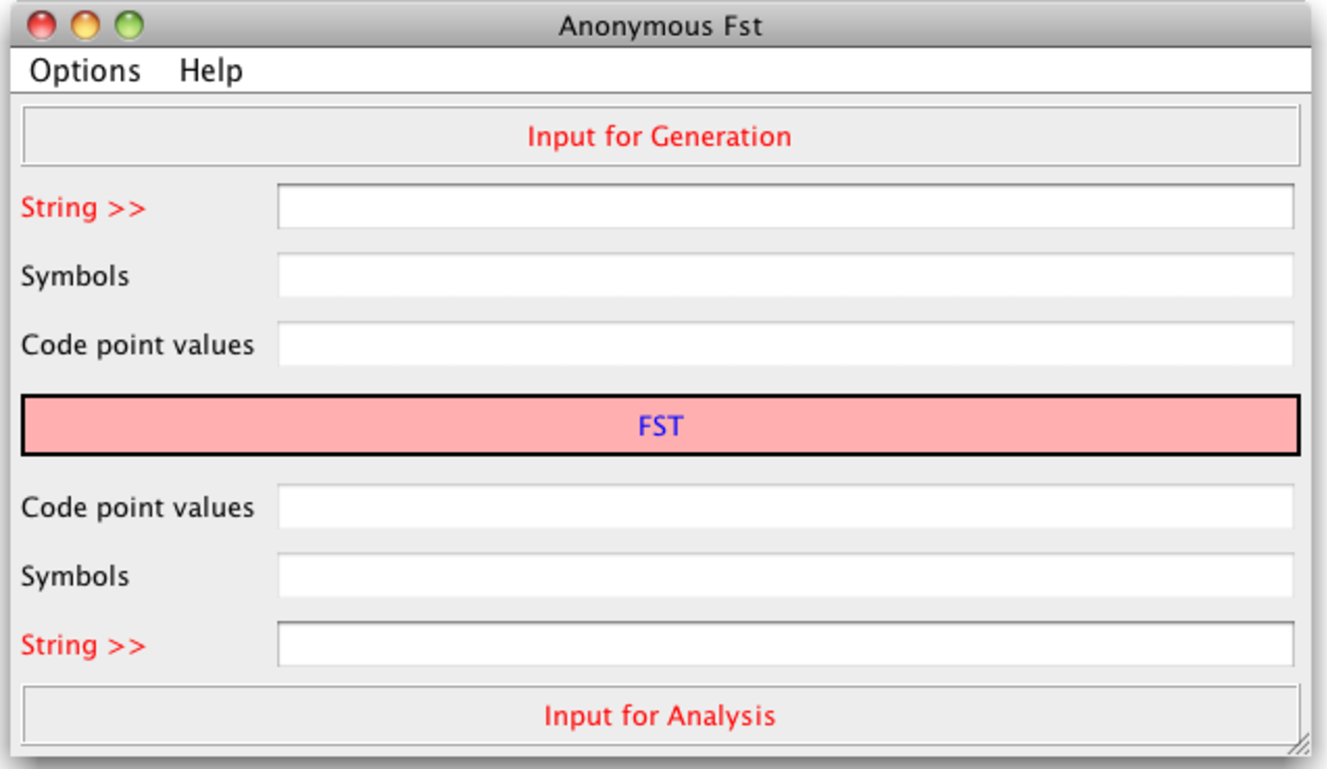
\includegraphics[width=\textwidth]{images/testWindow.pdf}
\end{center}

The testing window has an editable upper input field labeled
\emph{String >>} at the top and an editable lower input field (also
labeled \emph{String >>} at the bottom.  The
bar in the middle labeled ``FST'' represents the \acro{fst} being tested.  Type \emph{pacem} in the \emph{upper} field,
press the \key{enter} key, and the following output will appear in the \acro{gui} terminal window:


\begin{Verbatim}
pakem : 0.0
\end{Verbatim}

\noindent
Congratulations.  You have just written
and tested your first Kleene alternation rule.  For now don't worry about the ``0.0,'' which
represents a weight of zero, being the neutral weight
or the absence of weight.    Try testing this rule with a few more Latin words with \emph{c} such as
\emph{vici}, \emph{pecunia},
\emph{agricola}, \emph{victoria}.

Then experiment with the following Italian and Spanish rules.  Kleene can handle Unicode characters
like ʧ, and the \acro{gui} will display them if your Java installation has a font
that includes International Phonetic Alphabet glyphs, but for now you can substitute some other character or characters, e.g.


\begin{Verbatim}
// Italian, 
// using tS to represent the affricate like ch in chin
test  c -> tS / _  (e|i) ;
\end{Verbatim}

\begin{Verbatim}
// Spanish
test  c -> s / _  (e|i) ;
\end{Verbatim}


\noindent
Note also that if you enter

\begin{Verbatim}
$myrule =  c -> tS / _  (e|i) ;
\end{Verbatim}

\noindent
Kleene will display in the symbol-table window an icon, clearly labeled ``\$myrule,'' that represents the resulting
\acro{fst}.  If you right-click on that icon, a menu will appear, and you can select the \texttt{test} menu item to
cause the test window to be displayed.

[KRB:  add a graphic showing the pull-down menu.]

\subsection{Derivations or Cascades of Rules}

In the Italian and Spanish examples, there are actually two rules working together to describe the realizations of
\emph{c} in different contexts.  We'll look at the Spanish examples and refine them to be more correct and robust.  One
way to combine the rules together is via \emph{composition}, an
operation for which the syntactic 
operator is the Unicode \acro{ring operator}, \ringop{}, which
has the code point value U+2218.  Few fonts supply a glyph for this
character, so for now, and at any time, you can use
the \acro{ascii} equivalent \verb!_o_!, consisting of an
underscore, followed by a lowercase \emph{o} letter, followed by another underscore.\footnote{If you use the
Kleene.kmap input method, the typed \verb!_o_! sequence will be
intercepted and replaced with the \acro{ring operator} \ringop{}.}
Try entering the following derivation or ``cascade'' of rules and testing them using words like \emph{casa},
\emph{cosa}, \emph{poco}, \emph{curioso}, \emph{ciudad}, \emph{cace} and \emph{cimento}.


\begin{Verbatim}
// Two Spanish rules composed together
$rule = c -> s / _  (e|i) _o_ c -> k / _ (a|o|u) ;
test $rule ;
\end{Verbatim}

To better visualize the cascade of the two rules, they can equivalently be typed as

\needspace{5\baselineskip}
\begin{Verbatim}
// Two Spanish rules composed together
$rule = c -> s / _  (e|i) 
_o_ 
c -> k / _ (a|o|u) ;
test $rule ;
\end{Verbatim}

\noindent
and we will often talk about one rule, here the \texttt{c -> k} rule, being compose ``below'' or
``underneath'' the \texttt{c -> s} rule.  Recall that regular
expressions, including those with alternation-rule notations, can extend
over multiple lines and are always terminated with a semicolon.  When this cascade of rules is applied in a downward direction to an input
string, the output of the first (top) rule \verb!c -> s / _  (e|i)!
becomes the input to the second \verb!c -> k / _ (a|o|u)! rule
underneath it, and the output of the application is the output of the
final (here the second) rule.

Spanish speakers will note that the \texttt{c -> s} rule should also apply in the context
before the accented letters
\emph{é} and \emph{í}.  In addition, \emph{c} can also occur in environments not followed by a vowel,
and \emph{c} is realized as \emph{k} everywhere except before \emph{e}, \emph{é}, \emph{i} or \emph{í}.
To better capture the facts of Spanish pronunciation, 
we can simply add the accented variants to the context of the \texttt{c -> s}
rule, and remove the context altogether from the \texttt{c -> k} rule.  Intuitively, after the \texttt{c -> s}
rule has fired, any \emph{c}s still remaining will be mapped to \emph{k}.

\begin{Verbatim}
// Improved Spanish rules for the realization of c
$rule = c -> s / _  (e|é|i|í)
_o_
c -> k ;

test $rule ;
\end{Verbatim}

\noindent
The new rule cascade will now handle cases like \emph{pacto} and \emph{accidente},
outputting \emph{pakto} and \emph{aksidente}, respectively.  Note that if a rule does not ``match and fire,'' then it simply maps the input string to itself.  

[KRB:  add graphics showing the rule compiled into finite-state
machines]

As another example, consider the case of an imaginary language that has a
morpheme \emph{kaN}, terminating in an unspecified nasal consonant that we will
represent as uppercase \emph{N}, that can concatenate onto another morpheme
\emph{pat} to form the abstract string \emph{kaNpat}.  Let us assume that this language
has two alternation rules:

\begin{enumerate}
\item
The unspecified nasal \emph{N} is realized as \emph{m} before \emph{p} or
\emph{b}, and
\item
\emph{p} is realized as \emph{m} after \emph{m}, which might be an abstract
\emph{m} or an \emph{m} that was originally an \emph{N}.
\end{enumerate}

\noindent
These rules can be written, composed and tested in the \acro{gui} by entering


\begin{Verbatim}
$r = N -> m / _ (p|b)
_o_
p -> m / m _ ;
test $r ;
\end{Verbatim}

\noindent
and then entering \emph{kaNpat} as the upper-side input.  The output is the string
\emph{kammat}.  Intuitively, the downward application of the first \texttt{N ->
m} rule will map \emph{kaNpat} to the intermediate string \emph{kampat}, and then
the second \texttt{p -> m} rule will map from \emph{kampat} to \emph{kammat}.
However, when the two rules are compiled and composed, there is no longer an
intermediate level, and the resulting transducer maps \emph{kaNpat} to
\emph{kammat} in a single step.

Using the same transducer, if
you input the string \emph{kampat}, then intuitively the first rule will not match, and
will simply map \emph{kampat} to itself (an identity mapping), and then the second
rule will map from \emph{kampat} to \emph{kammat}.  But once again, the composed
rules result in a single two-level transducer that performs the mapping in a
single step.  Note also that if you input \emph{kammat}, then the result is again
\emph{kammat}.

At this point it is instructive to use the same transducer and apply it in an
\emph{upward} direction to the input \emph{kammat}.  To do this, simply enter
\emph{kammat} in the lower input field of the testing window.  The output will
consist of three strings:

\begin{itemize}
\item
kaNpat
\item
kampat
\item
kammat
\end{itemize}

\noindent
We get these three results because the \acro{fst} compiled from the two rules is a
two-level transducer that encodes a regular relation.  That relation maps an
upper-side \emph{kaNpat}, \emph{kampat} or \emph{kammat} to a lower-side
\emph{kammat}; so, looking at the relation in the other direction, it maps the
lower-side \emph{kammat} to the upper-side strings \emph{kaNpat}, \emph{kampat}
and \emph{kammat}.

So far we have experimented with individual rules, and simple cascades of two rules.
More generally, in the realm of regular languages and
regular relations, the upper string  is ``mapped'' into one or more 
lower strings via a set of ordered rules, which could number in the dozens or hundreds.  Between each
pair of rules, there will be a conceptual intermediate level.


\needspace{10\baselineskip}
\begin{Verbatim}
Upper Level
    Rule 1
Intermediate Level 1
    Rule 2
Intermediate Level 2
    Rule 3
Intermediate Level 3
    ...
    Rule n
Lower Level
\end{Verbatim}

\noindent
Formally speaking, the rule cascade represents a regular relation that
has the universal language as
the upper-level language, and all the intermediate languages, and the surface language, are all regular
languages as well.  The various rules, each one representing a regular relation, can be combined
together into a single two-level transducer via the composition operation

\begin{samepage}
\begin{Verbatim}
Upper Language
    Rule 1
      _o_
    Rule 2
      _o_
    Rule 3
      _o_
    ...
    Rule n
Lower Language
\end{Verbatim}
\end{samepage}

\noindent
and the result of the composition is a single two-level transducer that directly relates the upper
language and the lower language.  In the process of composition, all of the intermediate languages disappear.

\needspace{3\baselineskip}
\begin{Verbatim}
Upper Language
	FST
Lower Language
\end{Verbatim}


[KRB:  Fill out this section.]  Cite Panini.  Compare Chomsky-Halle Rewrite Rules, Perl substitution statements.
Johnson 1972.  Kaplan and Kay.  Karttunen and Kempe.  AT\&T.


\subsection{The Richness of Alternation-Rule Types}

Kleene provides a rich set, perhaps the richest set anywhere, of alternation-rule types
that can, in expert hands, be used to model a wide variety of linguistic phenomena.
Unavoidably, this richness is a challenge to the beginner, and I will try to show how
each rule type is typically used and which types are most commonly used.  The semantics
of alternation rules are elegant but occasionally hard to grasp, and their computational
implementation is one of the biggest challenges in any language like Kleene.

Like traditional Chomsky-Halle Rewrite Rules, and like Xerox/\acro{parc} Replace Rules,
multiple Kleene alternation rules can be written and ordered in a derivation or
\emph{cascade}.  Because each rule in the cascade compiles into a finite-state transducer,
the closure properties of such transducers allow us to compose the cascade of transducers
together into a single finite-state transducer that has the exact same behavior as the
original cascade, but which maps directly from input to output in a single step.  This
was one of key theoretical discoveries of Johnson.

In addition, there are various ways that Kleene alternation rules can be notated to
compile and apply in \emph{parallel},\footnote{Xerox/\acro{parc} Replace Rules offer a
limited capability for parallel composition, but the rule types (rule arrows) must be
exactly the same, which is not a restriction in Kleene.}  which is a key characteristic
of the ``two-level'' rules proposed by Koskenniemi's Two Level Morphology and implemented
in the now little-used Xerox/\acro{parc} twolc compiler.\footnote{Traditional two-level
rules continue to be popular at the University of Helsinki, which has re-implemented
twolc (\url{https://kitwiki.csc.fi/twiki/bin/view/KitWiki/HfstTwolC}).}  However, in Kleene parallel rules, the rules are not limited, as in traditional
Two Level Morphology, to constraining only pairs of single characters.

\section{Basic Mapping Rules}

\subsection{Right-Arrow Rules}

We will now start looking at alternation rules with a bit more rigor.  
The most common and useful alternation rules are obligatory right-arrow mapping rules, written using
the \texttt{->} or \texttt{→} arrow, which are
superficially similar to the classic ``Rewrite Rules'' of Chomsky \& Halle.

The simplest alternation-rule syntax in Kleene is

\begin{alltt}
\emph{upper} -> \emph{lower}
\end{alltt}

\noindent
where \emph{upper} and \emph{lower} are
arbitrarily complex regular expressions, though they are semantically limited to
denoting regular languages (that is, \emph{upper} and \emph{lower} cannot denote regular relations).
Thus the following rules are valid


\begin{Verbatim}
a -> b

dog -> Hund

ab*c+(d|e|f) -> x{2}y+z
\end{Verbatim}

\noindent
while the following, which have \emph{upper} or \emph{lower} expressions that denote regular relations
(transducers) are illegal.

\begin{Verbatim}
// Semantically illegal
a:b -> c

// Semantically illegal
n -> n:m

// Semantically illegal
e:i -> o:u
\end{Verbatim}


More precisely, the \emph{upper} and \emph{lower} expressions must be interpretable as denoting
languages.  Recall that OpenFst finite-state machines are always two-level, with each arc having an
upper symbol and a lower symbol.  So each finite-state machine is implemented as a transducer, and
acceptors are special cases of such machines where, on every arc, the upper and lower symbols are the
same.  Thus the regular expression \texttt{b}, and the regular expression \texttt{b:b} are structurally
equivalent---they both get interpreted to produce an \fsm{} with one arc that has a \emph{b} symbol on
the upper side and a \emph{b} symbol on the lower side.  By convention, this machine is interpretable
as an acceptor.

Consistent with that convention, the following rules are valid because both the \emph{upper} and
\emph{lower} expressions are interpretable as denoting regular languages (not relations).

\begin{Verbatim}
// Syntactically and semantically legal, 
//    equivalent to a -> b
a:a -> b:b

// Syntactically and semantically legal, 
//    equivalent to dog -> chien
d:d o:o g:g -> c:c h:h i:i e:e n:n

(dog):(dog) -> (chien):(chien)
\end{Verbatim}

\noindent
But if either the \emph{upper} expression or the \emph{lower} expression cannot be interpreted as
denoting a regular language, an exception will be thrown at runtime.

Alternation rules can also be constrained to match and ``fire'' only in a specified context, based on
the following template, where \emph{upper}, \emph{lower}, \emph{left} and \emph{right} can all be
arbitrarily complex regular expressions, but all are semantically limited to be interpretable as
regular languages.  The left-hand-side of the rule is separated from the context (which is the
right-hand-side) by a forward slash \texttt{/}. The underscore
character \texttt{\_} marks the position in the context where the \emph{upper} expression appears.
 

\begin{alltt}
\emph{upper} -> \emph{lower} / \emph{left} _ \emph{right}
\end{alltt}

\noindent
When such a rule is applied ``in a downward direction'' to an input string, the input string must match the \emph{left}
context, the \emph{upper} expression and the \emph{right} context in order for the rule to fire; if the rule does match the input, then the
\emph{upper} content on the upper side is mapped to the \emph{lower} content in the output(s).  If the
input is not matched by the rule, then the rule simply maps the input to itself, the identity mapping.


The use of the underscore character to separate the left context from the right context signals the
Kleene interpreter that the rule writer intends the context to be interpreted as one-level, i.e.\@ the
\emph{left} and \emph{right} context expressions denote regular languages and are to be matched on the upper
side of the relation.  As we shall see, Kleene alternation rules based on Huldén's algorithms can
also have two-level contexts, denoting transducers; but there is such a long tradition of rules with
single-level contexts that Kleene retains this traditional syntax for the traditional semantics.  If
the programmer genuinely intends to designate two-level contexts, then that will be signaled by a
slightly different syntax to be presented below.  For now we will concentrate on basic mapping rules
wherein all the rule parts---upper, lower, left context and right context---are intended
by the programmer
to denote regular languages, and where the accidental definition of a two-level context will be caught
and signaled as an error.

The following rule examples are illegal because the contexts are two-level:

\begin{Verbatim}
// Semantically bad rules
a -> b / q:r _ s:t

a -> b / q:r _

a -> b / _ s:t
\end{Verbatim}

\noindent
The contexts can consist of or contain variables previously defined, and they must denote regular languages.


\begin{Verbatim}
// Semantically good
$left = qrst ;
$right = xyz ;

$r = a -> b / $left _ $right ;
\end{Verbatim}

\noindent
If either context part cannot be interpreted as a regular language (an acceptor), then the rule is semantically bad and
a runtime exception will be thrown.  As the following example illustrates, illegal two-sided contexts can in general be detected
only at runtime, when the context expressions are evaluated.  This is similar to the way that illegal division by zero
must be detected in general-purpose programming languages.

\begin{Verbatim}
// Semantically bad
$left = (qr):(st) ;
$firht = x:y ;

a -> b / $left _ $right ;  // a runtime exception will be thrown
\end{Verbatim}


Although an overall alternation rule compiles into a two-level transducer that could be applied either in an
upward or a downward direction, right-arrow rules have a clear downward bias to them;
we normally think of the upper level of a two-level rule as the input side of the
relation.  (This notion of input side corresponds with the OpenFst visualization of a
machine's ``input'' side.)
In such a basic right-arrow rule, the input expression and both the left
and right context expression must match on the upper side of the relation.

As a concrete example, the following rule, intended to model a phenomenon in Italian and Portuguese
pronunciation of written words, maps \emph{s} to \emph{z} in the context between two vowels.


\begin{Verbatim}
s -> z / (a|e|i|o|u) _ (a|e|i|o|u)
\end{Verbatim}

\noindent
This particular rule could be written equivalently as


\begin{Verbatim}
s -> z / [aeiou] _ [aeiou]
\end{Verbatim}

\noindent
Either way, this rule would map, in a downward direction, from \emph{casa} to \emph{caza}, \emph{mesa} to \emph{meza},
\emph{isose} to \emph{izoze}, etc.

The syntactic contexts in alternation rules are optional, allowing the following variations:

\begin{alltt}
\emph{upper} -> \emph{lower} / \emph{left} _ \emph{right} // both contexts present
\emph{upper} -> \emph{lower} /     _ \emph{right}         // right context only
\emph{upper} -> \emph{lower} / \emph{left} _              // left context only
\emph{upper} -> \emph{lower}                              // no contexts
\end{alltt}

\noindent
A missing context is semantically equivalent to \verb!.*!, the Universal Language, e.g.

\begin{alltt}
\emph{upper} -> \emph{lower} /    _ \emph{right}	    // right context only
\emph{upper} -> \emph{lower} / .* _ \emph{right}	    // equivalent
\end{alltt}


Alternation rules can have multiple contexts, separated by \texttt{||}, a double vertical bar.

\begin{alltt}
\emph{input} -> \emph{output} / \emph{L1} _ \emph{R1} || \emph{L2} _ \emph{R2} \ldots
\end{alltt}

\subsection{Left-arrow Rules}

Left-arrow rules, using the \texttt{<-} arrow, are similar to right-arrow
rules but have a default bottom-up orientation or reading.

\begin{Verbatim}
z <- s / [aeiou] _ [aeiou]
\end{Verbatim}

\noindent
In a left-arrow rule, it is natural to think of the lower side as being the input side,\footnote{Recall,
however, that in the OpenFst visualization of transducers, the upper side is always termed the ``input
side'' and the lower side is always termed the ``output side.''} and in this example the
\emph{s} and
the two contexts would need to match the lower-side input for the rule to fire.  If this rule is
applied ``in an upward direction'' to the lower-side input string \emph{casa}, the upper-side output
is \emph{caza}.  You can test this in the \acro{gui} in the usual way:


\begin{Verbatim}
$leftrule = z <- s / [aeiou] _ [aeiou] ;
test $leftrule ;
\end{Verbatim}

\noindent
and then enter a string like ``casa'' in the \emph{lower} input field of the test window.


Experts in finite-state programming are often quick to point out that left-arrow rules
are technically unnecessary.  The composition

\begin{Verbatim}
$result = z <- s / [aeiou] _ [aeiou] 
_o_ 
$fst ;
\end{Verbatim}

\noindent
which composes a left-arrow rule ``on top of'' an existing machine bound to \verb!$fst!,
could be accomplished equivalently, without left-arrow rules, by 

\begin{itemize}
\item
Writing the alternation as a right-arrow rule:  \verb!s -> z / [aeiou] _ [aeiou]!
\item
Inverting the \verb!$fst!:  \verb!$^invert($fst)!
\item
Composing the right-arrow rule on the lower side of the inverted \verb!$fst!:
\verb!$^invert($fst) _o_ s -> z / [aeiou] _ [aeiou]!
\item
And then inverting the result:\\ 
\verb!$^invert($^invert($fst) _o_ s -> z / [aeiou] _ [aeiou])!
\end{itemize}


\noindent 
While all that inversion makes perfect sense in theory, many find it less than intuitive to write grammars that way.
Users will have to judge for themselves whether to use
the formally unnecessary left-arrow rules.

\section{Optional Alternation Rules}

A right-arrow rule using the \texttt{→?} or \texttt{->?} arrow (a normal right arrow followed by a question
mark\footnote{In regular expressions, the question mark is a postfix operator indicating the optionality of the expression that
precedes it.  In a similar spirit, adding a question mark after a rule operator signals that the mapping indicated by the rule is
optional.}) applies optionally.  Thus
the rule

\begin{Verbatim}
s ->? z / [aeiou] _ [aeiou]
\end{Verbatim}

\noindent
maps the upper-side input string \emph{casa} to two outputs, \emph{caza} (representing the output when
the rule matches and fires) and
\emph{casa} (representing the output when the rule doesn't fire).  It 
maps the string \emph{isose} to four outputs:
\emph{izoze}, \emph{izose}, \emph{isoze} and \emph{isose}.

Similarly, a left-arrow rule using the \texttt{←?} or \texttt{<-?} arrow (a normal left arrow followed by a question mark) also
applies optionally, but in a bottom-up orientation.

\begin{Verbatim}
z <-? s / [aeiou] _ [aeiou]
\end{Verbatim}

\section{Maximum and Minimum Matching}

Straightforward mapping rules will match and apply in all possible ways, with multiple outputs
whenever there are multiple ways to match the input.  [KRB:  Add an example.]  In practice, it is often useful to write rules that act as
if a matching algorithm were moving left-to-right through the input string, always matching the
	maximum numbers of symbols whenever two or more matches are possible.  The syntax for such rules
	adds \verb!{max}! to the arrow:

\begin{alltt}
\emph{upper} \{max\}-> \emph{lower} / \emph{left} _ \emph{right}
\emph{upper} <-\{max\} \emph{lower} / \emph{left} _ \emph{right}
\end{alltt}

\noindent
Note that the \verb!{max}! appears next to the input expression, which is the upper side in a right-arrow rule, and the lower side
in a left-arrow rule.

[KRB: add concrete example of syllabification]  

It is important to understand that although the behavior of these rules appears to move
left-to-right, and looks like some kind of algorithm is being performed at runtime, these
rules, like all the other alternation rules, are compiled into finite-state transducers
that encode a regular relation.

In some cases, it is also useful to write rules that again act as if a matching algorithm
were moving left-to-right through the input string, but which always match the
\emph{minimum} rather than the maximum if multiple matches are possible.  In such rules a
\verb!{min}! is added to the arrow:

\begin{alltt}
\emph{upper} \{min\}-> \emph{lower} / \emph{left} _ \emph{right}
\emph{upper} <-\{min\} \emph{lower} / \emph{left} _ \emph{right}
\end{alltt}

[KRB:  consider implementing similar rules with apparent right-to-left
behavior, similar to the Xerox ->@ and >@ rules.  2013.  Direct
implementation of such rules would appear to require modifications of
Hulden's algorithms.]


\section{Epenthesis Rules}

An epenthesis rule inserts symbols where no symbols were before.  That it, it matches the empty string and maps it to
something not empty.  Recall that empty double quotes, \verb!""!, denotes the empty string.  The following epenthesis rule

\begin{Verbatim}
"" -> i /  p _ t
\end{Verbatim}

\noindent
maps the upper string \emph{apto} to the lower string \emph{apito}.  Technically speaking, there are an infinite number
of empty strings between any two adjacent symbols like \emph{p} and \emph{t}, and at the beginning and end of a string, and such rules might have been interpreted to force
an infinite number of outputs.\footnote{The Xerox replace rule intuitively written \verb!0 -> i || p _ t! is indeed interpreted this
way and results in an error.  Xerox epenthesis rules must be notated with special ``dotted brackets,'' 
e.g.\@ \verb![..] -> i || p _ t! to avoid the error.}  However, the intent of a programmer who writes \verb!"" -> i /  p _ t! is almost always to
interpret the input as having only one empty string between symbols, and at the boundaries of a string, and the Kleene rule is automatically interpreted in this way.


\section{Markup Rules}

Markup rules match an input expression, map that input expression to itself in the output, and then ``mark up'' the
output by surrounding it with symbols specified in the rule, e.g.

\begin{Verbatim}
[aeiou] -> '<v>' ~~~ '</v>'
\end{Verbatim}

\noindent
where the intent is to surround each vowel in the output with the \acro{xml}-like symbols \verb!<v>! and \verb!</v>!.  Applied downward,
this rule will map \emph{unique} to \emph{<v>u</v>n<v>i</v>q<v>u</v><v>e</v>}.

\section{Two-Level Rule Contexts}

Using Huld\'en's algorithms, it became possible to implement alternation rules with two-level contexts.\footnote{Two-level contexts
were not possible in Xerox Replace Rules.}
Compare the following examples:

\begin{Verbatim}
a -> b / b _
\end{Verbatim}

\noindent
is a rule with a one-level context, and it maps \texttt{baaa} downward to \texttt{bbaa}, while

\begin{Verbatim}
a -> b / (.*):b _2_
\end{Verbatim}

\noindent
is a rule with a two-level context that maps \texttt{baaa} to {bbbb}.  The
\verb!_2_! syntax indicates that the context or contexts are to be interpreted as
having two levels.  Here the left context is \verb!.*! (the Universal Language) on the upper side and \verb!b! on the
lower side.

[KRB:  explain, step by step, how the only possible output is bbbb]

This kind of rule, where the left-context matches on
the lower side of the relation, appears to generate its own left context as it moves
along, resulting in a kind of left-to-right domino effect.  However, it is
important to realize that there is no algorithm or process being performed; the rule,
like all alternation rules, is compiled into a static finite-state transducer, a data
structure that encodes a
relation between two regular languages.  The output only appears to reflect a kind of
left-to-right domino effect that generates its own lower-side left contexts as it
moves along.

In natural-language phonetics and morphology, such rules are often used to model a phenomenon known
as vowel harmony.  [Give examples.]

In a similar way, note that

\begin{Verbatim}
a -> b / _ b
\end{Verbatim}

\noindent
maps \texttt{aaab} to \texttt{aabb}, while

\begin{Verbatim}
a -> b / _2_  (.*):b
\end{Verbatim}

\noindent
maps \texttt{aaab} to \texttt{bbbb}.  Here again, the \verb!_2_! operator indicates that the context or contexts are to
be interpreted as having two levels, and here the right context is \verb!.*! on the upper side and \verb!b! on the lower
side.  The rule with a two-level right context appears to
operate right-to-left, generating its own lower-side right context as it moves along, outputting \texttt{bbbb} in a kind
of right-to-left domino effect.
Again, the rule really just compiles into a finite-state transducer that encodes a regular
relation, and there is no runtime algorithm or process involved.
Such rules have been found useful to model a phenomenon known as umlaut.

The following example of maximal matching involves the insertion of a hyphen to mark a syllable-boundary
marker, where a syllable starts with a
consonant, continues with one or more vowels and ends with zero or more consonants,
provided that the right context starts with one consonant and a vowel.\footnote{Thanks to
Lauri Karttunen for this example.}

\begin{Verbatim}
// Define a set of consonants for your language
// 	(modify as necessary)
$C = [bcdfghjklmnprstvyz] ;

// Define a set of vowels for your language
$V = [aeiou] ;

// Define a syllable as the maximal match of
//	one consonant, followed by
//	one or more vowels, followed by
//	zero or more consonants, provided that
//	it is followed by one consonant and a vowel.
// Insert a hyphen after such a matched syllable.
$Syll = $C $V+ $C* {max}->   ~~~ "-" / _ $C $V ;

// Define a convenient function that 
//	takes an input string,
//	apples $Syll to the string in a downward direction, and
//	returns the lower side of the resulting relation.
$^Syllabify($str) { 
	return $^lowerside($str _o_ $Syll) ; 
}

// Syllabify an input string.  Use double quotes
//	to literalize the space.
$words = $^Syllabify("lauri karttunen") ;
print $words ;	
// => lau-ri kart-tu-nen : 0.0

// Syllabify another word, bypassing the $words variable.
//	No double quotes are needed here.
print $^Syllabify(continental) ;
// => con-ti-nen-tal
\end{Verbatim}

\section{Parallel Rules}

\subsection{Vertical Derivations vs.\@ Parallel Rules}

So far we have combined multiple rules in vertical derivations (cascades), and this
approach is often natural and intuitive.  In such derivations, the relative orders of some
rules can be critical, and there are classic cases where rule ordering causes challenges
that can be overcome only with ugly kludges.  For example, consider the case where we want
a rule (or set of rules) to take the input string \emph{abba} and return the string
\emph{baab}; and for the input \emph{baab}, we want the output \emph{abba}.  Similarly,
\emph{aaaaa} should map to \emph{bbbbb}, and \emph{ababaa} should map to \emph{bababb}.  In
short, we want every \emph{a} to be mapped to \emph{b}, and we want every \emph{b} to be
mapped to \emph{a}.  Instinctively, we imagine two trivial rules:


\begin{Verbatim}
a -> b 
\end{Verbatim}

\noindent
and

\begin{Verbatim}
b -> a
\end{Verbatim}

As a first attempt, we try to compose the two rules with the \verb!a -> b! rule above the
\verb!b -> a! rule, and we define a trivial function \verb!$^swap! to facilitate testing.


\begin{Verbatim}
$deriv =  a -> b
          _o_
          b -> a ;
$^swap ($word) { 
    return $^lowerside($word _o_ $deriv) ;
}

print $^swap(abba) ;
// => aaaa
\end{Verbatim}

\noindent
To our disappointment, when we apply \verb!$^swap! to \emph{abba}, the output is not the desired
\emph{baab} but rather the string \emph{aaaa}.  We then try the opposite ordering of the
two rules

\begin{Verbatim}
$deriv =  b -> a
          _o_
          a -> b ;
$^swap ($word) { 
    return $^lowerside($word _o_ $deriv) ;
}

print $^swap(abba) ;
// => bbbb
\end{Verbatim}

\noindent
and the output this time is \emph{bbbb}, again not the desired \emph{baab}.  The problem
can be traced by imagining the two rules apply separately.  In the first case, with the
ordering


\begin{Verbatim}
$deriv =  a -> b
          _o_
          b -> a ;
\end{Verbatim}

\noindent
the first rule will map \emph{abba} to \emph{bbbb}, and then the second rule will map
\emph{bbbb} to \emph{aaaa}.  In the second case, with the ordering


\begin{Verbatim}
$deriv =  b -> a
          _o_
          a -> b ;
\end{Verbatim}

\noindent
the first rule will map \emph{abba} to \emph{aaaa}, and then the second rule will map
\emph{aaaa} into \emph{bbbb}.  Obviously, one rule is undoing the work
of the other, and simple ruler e-ordering will not solve this
problem.

In ordered derivations, such problems can be solved by the use of a temporary symbol---we
will use the multicharacter symbol \verb![TEMP]!---in the following way


\begin{Verbatim}
$deriv =  a -> '[TEMP]'
          _o_
          b -> a
          _o_
          '[TEMP]' -> b ;

$^swap($word) {
    return $^lowerside($word _o_ $deriv) ;
}

print $^swap(abba) ;
// => baab
\end{Verbatim}

\noindent
but this is far from beautiful or intuitive.  Instinctively, we just want to write our two
simple rules, \verb!a -> b! and \verb!b -> a!, and specify somehow that they are to be
applied in parallel, simultaneously, rather than one ordered after the other.  

\subsection{The Built-In Parallel Function}

\subsubsection{The abba Example}

Huld\'en's algorithms allow alternation rules to be compiled in parallel with complete freedom [KRB:  test and confirm
this].  Unlike xfst Replace Rules, which can be compiled in parallel only if they have the exact same arrow operator,
Kleene allows rules of any arrow type to be compiled in parallel.  Unlike traditional Two-Level alternation rules, which are
compiled in parallel but are
limited to controlling the mapping of one symbol to one symbol (the so-called ``concrete pairs''), Kleene allows
rules with arbitrary-length mappings to be compiled in parallel.

The overt way to indicate that a set of rules is to be compiled in parallel is to enclose them in the \verb!$^parallel()!
built-in function, separated by commas.  Our problematic \emph{abba} example shown just above
can be formulated straightforwardly as

\begin{Verbatim}
$r = $^parallel(a -> b, b -> a) ;

#^swap($word) {
    return $^lowerside($word _o_ $r) ;
}

print $^swap(abba)
// => baab

print $^swap(baab)
// => abba

print $^swap(ababaa)
// => bababb
\end{Verbatim}

\noindent
By compiling the \texttt{a -> b} and \texttt{b -> a} rules in parallel, they apply simultaneously and give us the desired
results.
The resulting machine will map \emph{abba} to \emph{baab}, \emph{baab} to \emph{abba},
etc. 


Proponents of parallel rules, notably Professor Kimmo Koskenniemi of the University of
Helsinki, argue that parallel rule compilation is inherently simpler than ordered
derivations.  They emphasize the difficulties of rule ordering and point out that a
developer must understand and somehow keep track of all the intermediate levels in a
derivation.  However, non-trivial sets of rules applied in parallel can conflict in
various ways that are not at all easy for most developers to understand and fix,
especially where the rule set includes deletions or epentheses; and writing rules in parallel
also often requires the careful use of two-level contexts, often specifying that one side
of the context must match while the other side can be anything (the universal language).

Consider the case of the \emph{kaNpat} example, previously encoded as a cascade 

\begin{Verbatim}
$r = N -> m / _ (p|b)
_o_
p -> m / m _ ;
test $r ;
\end{Verbatim}

\noindent
Using parallel rules, this example can also be encoded equivalently as

\begin{Verbatim}
$r = $^parallel( N -> m / _ (p|b) , p -> m / (.*):m _2_ ) ;
test $r ;
\end{Verbatim}

\noindent
where the \texttt{p -> m} rule now has a left context \texttt{(.*):m} that matches
anything (the universal language) on the upper side but \emph{m} on the lower
side.  This is effectively the way of saying that the \texttt{m} of the left context could
be an original input \emph{m}, or it could be something (a symbol, a sequence of symbols,
or perhaps even the empty string) that is being mapped to \emph{m} by
any one of the other rules
being compiled in parallel.  

Consider also the mapping of Brazilian-Portuguese \emph{time} to \emph{tSimi} and \emph{parte} to \emph{partSi}, done earlier using a cascade of rules.  


\begin{Verbatim}
$r = e -> i / _ #
_o_
t -> tS / _ i ;
\end{Verbatim}

\noindent
The same mappings can be performed by two rules compiled in parallel.

\begin{Verbatim}
$r = $^parallel( e -> i / _ # ,  t -> tS / _2_ (.*):i ) ;
\end{Verbatim}

\noindent
In this case, the right context of the \texttt{t -> tS} rule must be written as the
two-level \texttt{(.*):i}, indicating that the \emph{i} could be an original input
\emph{i} or something mapped to \emph{i} by another parallel rule.  Writing such two-level
contexts correctly is not always easy for developers.  

Consider also the following example, which (in a rule with one-level contexts) maps
\emph{a} to \emph{b} in the context between \emph{c} and
\emph{d}, and also, in a rule with two-level contexts, maps \emph{d} to \emph{e} after an
\emph{a} that has been simultaneously mapped to a \emph{b} by the first rule.  These rules compile
in parallel to a machine that maps \emph{cad} to \emph{cbe}.

\begin{Verbatim}
$r = $^parallel( a -> b / c _ d ,  d -> e / a:b _2_ ) ;
\end{Verbatim}

In general, every rule compiled in parallel must ``be aware'' of what all the other rules
in the parallel-rule set are doing.  More precisely, the writer of each rule must be aware of
what all the other rules in the parallel-rule set are doing
simultaneously.  Where there are only two or a few rules,
as in these examples, the challenge may seem trivial; but in real-life systems, there may
easily be
dozens of rules, and conceiving the effect of all of them operating simultaneously is
challenging, to say the least.

There is no mathematical basis for choosing to write rules in a vertical cascade vs.\@ in
parallel---the result is always regular in power, encodable as a finite-state transducer.
Some examples will seem easier to encode one way or the other, and different developers
will have differing conceptual capabilities and tastes.  Kleene allows rule sets to be
encoded as derivations, in parallel, or in a mixture of the two approaches.

Note that \verb!$^parallel()! is a special built-in function that requires that its arguments be in full rule syntax.  The following example, which
tries to compile the rules separately into finite-state machines, and then pass
the machines as arguments to \verb!$^parallel()! is syntactically and
semantically
illegal.  In order to compile rules in parallel, the Huld\'en algorithms need to access
and compile all of the original rule parts,
combining them together in non-trivial ways.  If a rule has been pre-compiled into a finite-state machine, the original parts of
the component rules are no longer identifiable or extractable.

\begin{Verbatim}
$rule1 = e -> i / _ # ;
$rule2 = t -> tS / _2_ (.*):i ;

// this is ILLEGAL
$r = $^parallel( $rule1 ,  $rule2 ) ;

// while this is legal
$r = $^parallel( e -> i / _ #, t -> tS / _2_ (.*):i ) ;
\end{Verbatim}

\subsection{Rules with Where Clauses}

\subsubsection{The Devoicing Example}

Kleene alternation rules can also have \emph{where}-clause directives that define the settings of local variables inside the rules.  The following rule

\begin{Verbatim}
$r = $voiced -> $unvoiced / _ # 
          {where  $voiced _E_ $@(b, d, g), 
                  $unvoiced _E_ $@(p, t, k) } ;
\end{Verbatim}

\noindent
models the phenomenon where voiced consonants become devoiced at the end of a word.  (The rule is written on multiple lines to be
more readable, but this is not required.) In German, as a real-world example, the word
written \emph{Tag} is pronounced \emph{Tak}, the word written \emph{Hund} is pronounced
\emph{Hunt}. etc.  This rule is effectively expanded to
three rules that are compiled in parallel, equivalent to

\begin{Verbatim}
$r = $^parallel( b -> p / _ #, 
                 d -> t / _ #, 
                 g -> k / _ # ) ;
\end{Verbatim}

\noindent
In this case, the \texttt{{where ...}} clause defines two local variables,
\verb!$voiced! and \verb!$unvoiced!, each of which is bound to a value, one at a
time, from a supplied list of finite-state machines.  The finite-state machines can be
arbitrarily complex, though they must conform to any semantic limitations
inherent to rules; in this example, \verb!$voiced! and \verb!$unvoiced! appear on
the left-hand-side of the rule, where the expressions must denote regular
languages (not relations).  By default, as in this case, the local variables are
bound, during interpretation, to the list values in a left-to-right ``matched''
fashion such that when \verb!$voiced! is bound to its first value \verb!b!, \verb!unvoiced! is
bound to its first value \verb!p!, and when \verb!$voiced! is bound to \verb!d!, \verb!unvoiced!
is bound to \verb!t!, etc.  This matched assignment behavior requires that the
two list expressions have exactly the same length, and Kleene will throw an
exception if they are not.  

Where-clauses can define one, two or more variables that are interpreted as being
local to the rule.\footnote{The Kleene interpreter literally pushes to a new
frame/scope while compiling a rule with where-clauses, so that resetting the
values of the local rule variables does not effect any variables outside the rule
that happen to have the same names.}  Each local variable in the where-clause is
followed by the ``element of'' operator, which can be the $\in$ character
(Unicode \acro{element of}, U+2208) or the \acro{ascii} equivalent \verb!_E_!.  The
syntax \verb!$@(...)! is the normal Kleene syntax for a literal anonymous list of
finite-state-machine values.  After the $\in$ or \verb!_E_! can appear any Kleene
expression whose value is a list of finite-state machines, including variables
and even function calls that return such a list.

\begin{samepage}
\begin{Verbatim}
$@voicedstops = $@(b, d, g) ;
$@unvoicedstops = $@(p, t, k) ;

$r = $voiced -> $unvoiced / _#  
        {where  $voiced   _E_ $@voidedstops, 
                $unvoiced _E_ $@unvoicedstops } ;
\end{Verbatim}
\end{samepage}

\noindent
The following rule, which doubles all vowels, e.g.\@ mapping \emph{unido} to
\emph{uuniidoo}, calls \verb!$@^getSigma()!, which is a pre-defined function that
calculates the alphabet (the sigma) of its
argument and returns it as a list of finite-state machines.

\begin{Verbatim}
$r = $vowel -> $vowel $vowel 
          { where  $vowel _E_ $@^getSigma(aeiouAEIOU) } ;
\end{Verbatim}

\subsubsection{The Caesar Cipher Example}

Julius Caesar employed a simple-substitution cipher wherein each Latin letter was replaced by the letter three steps down
in the alphabet, e.g.\@ A was replaced by D, B was replaced by E, C was replaced by F, etc.  At the end of the alphabet,
the mapping ``wrapped around'' to the beginning so that X was replaced by A, Y by B and Z by C.  Like the abba example
above, we intuitively just want all the letter substitutions to happen simultaneously, without mutual interference, and
this is another classic example were parallel compilation is desirable.  The following script uses the common convention
of treating the ``plaintext'' as consisting only of lowercase letters, and the ``ciphertext'' as consisting only of uppercase
letters.  Arbitrarily, the script is written to ``generate'' (apply downwards) from a plaintext string to the
corresponding ciphertext strings.


\begin{Verbatim}
$@plainletter =  $@(a,b,c,d,e,f,g,h,i,j,k,l,m,n,o,
                    p,q,r,s,t,u,v,w,x,y,z) ;
$@cipherletter = $@(D,E,F,G,H,I,J,K,L,M,N,O,P,Q,R,
                    S,T,U,V,W,X,Y,Z,A,B,C) ;

$en = $pl -> $cl {where $pl _E_ $@plainletter,
                        $cl _E_ $@cipherletter} ;

$^encipher($plain) {
    return $^lowerside($plain _o_ $en) ;
}

print $^encipher("attack at dawn") ;
// => DWWDFN DW GDZQ: 0.0
\end{Verbatim}



The script begins with the definition of \texttt{\$@plainletter} as a list that contains all the plaintext letters in
normal alphabetical order.  \texttt{\$@cipherletter} is then defined as a list of ciphertext letters starting with \emph{D},
reflecting Caesar's original offset.
\texttt{\$en} is a rule that maps each plaintext letter to its corresponding ciphertext letter, and \verb!$^encipher! is a
little function that composes the \verb!$en! rule ``under'' the input string and then extracts and returns the lower side
(the output) of the result.  The result of \verb!$^encipher("attack at dawn")! is the ciphertext \emph{DWWDFN DW GDZQ}.

There are two ways to implement decipherment of the same cipher.  Following the same pattern, we can define \verb!$de! as
a rule that maps each ciphertext letter to its plaintext equivalent, and the \verb!$^decipher! function facilitates the
testing to map \emph{DWWDFN DW GDZQ} back into the original \emph{attack at dawn} message.

\begin{Verbatim}
$de = $cl -> $pl {where $cl _E_ $@cipherletter,
                        $pl _E_ $@plainletter} ;

$^decipher($cipher) {
    return $^lowerside($cipher _o_ $de) ;
}

print $^decipher("DWWDFN DW GDZQ") ;
// => attack at dawn: 0:0
\end{Verbatim}

However, because the original \verb!$en!, defined as


\begin{Verbatim}
$en = $pl -> $cl {where $pl _E_ $@plainletter,
                        $cl _E_ $@cipherletter} ;
\end{Verbatim}

\noindent
maps downward from plaintext to ciphertext, and because we remember that regular transducers are in fact bidirectional, it
is tempting to avoid the definition of \verb!$de! and just use \verb!$en! to implement \verb!$^decipher! thus


\begin{Verbatim}
$^decipher($cipher) {
    return $^upperside($en _o_ $cipher) ;
}
\end{Verbatim}

\noindent
that is, to compose the cipher string on the \emph{lower} side of \verb!$en! and return the \emph{upper} side of the
result.  However, if we try to do that, each letter on the lower side, such as \emph{D}, will map upward to itself or to its
plaintext equivalent, here \emph{a}, and even for this short text there will be over a hundred outputs, reflecting all the
possible upward mappings.  Recall that such
a right-arrow rule has a downward orientation:  it states that an \emph{a} on the upper side maps to a \emph{D} on the
lower side, but it doesn't say that a \emph{D} on the lower side has to map to an \emph{a} on the upper side.  Because we
defined the problem in a way that the intended upper alphabet is all lowercase, and the intended lower alphabet is all
lowercase, we can fix
this particular example by simply constraining \verb!$en! not to contain any ciphertext (uppercase) letters on the upper side.

\begin{Verbatim}
$en = ~$contains([A-Z])
	_o_
	$pl -> $cl {where $pl _E_ $@plainletter,
                      $cl _E_ $@cipherletter} ;
$^decipher($cipher) {
    return $^upperside($en _o_ $cipher) ;
}
print $^decipher("DWWDFN DW GDZQ") ;
// =>  attack at dawn: 0:0
\end{Verbatim}

\noindent
This is a good reminder that while alternation rules compile into transducers, and transducers are bi-directional, a
right-arrow rule constrains the mapping only from the upper side to the
lower side, not vice versa.  Conversely, a left-arrow rule constrains
the mapping only from the lower side to the upper side, not vice versa.

\subsubsection{Deletion Rules}

\subsubsection{Where Mixed Clauses}

Kleene also supports the \verb!where mixed! keyword, which causes the interpreter to compute the Cartesian Product
of all the list values and assign the local variables to each of the
results in turn.  For \verb!where mixed!, the lists of values do not have
to have the same length.  For example, in the rule

\begin{Verbatim}
$r = $foo -> $bar 
      { where mixed $foo _E_ $@(a, b, c), 
	                $bar _E_ $@(y, z) } ;
\end{Verbatim}

\noindent
the Cartesian product of the values contains the six pairs (a, y), (a, z), (b, y), (b, z), (c, y) and (c, z), and so
the single rule is equivalent to the following six rules compiled in parallel:

\begin{Verbatim}
$r = $^parallel( a -> y, 
                 a -> z, 
                 b -> y, 
                 b -> z, 
                 c -> y, 
                 c -> z) ;
\end{Verbatim}

\noindent
and either rule will map upper-side input \emph{cab} to \emph{yyy}, \emph{yyz}, \emph{yzy}, \emph{yzz}, \emph{zyy}, \emph{zyz},
\emph{zzy} and \emph{zzz}.


Kleene also supports the \verb!where matched! keyword, equivalent to \verb!where!, if the
programmer desires to make the matched-assignment behavior more explicit.

\begin{Verbatim}
$r = $voiced -> $unvoiced / _ #
        { where matched $voiced   _E_ $@(b, d, g), 
                        $unvoiced _E_ $@(p, t, k) } ;
\end{Verbatim}

\noindent
In addition, one can write a rules with multiple where-clauses, potentially mixing \verb!where! (or
\verb!where matched!) and \verb!where mixed! clauses, and the interpreter will compute the Cartesian product of values
among the multiple where-clauses.  As the semantics quickly become opaque to the human programmer, multiple where-clauses are best avoided.

\subsection{Rules where the Input can Match the Empty String}

We have already examined epenthesis rules such as

\begin{Verbatim}
"" -> i / p _ t
\end{Verbatim}

\noindent
where the upper-side input expression is the empty string.  A similar case is where the input expression denotes a
language that includes the empty string, e.g.

\begin{Verbatim}
a* -> x / l _ r
\end{Verbatim}

\noindent
Note that \verb!a*! denotes a language that includes the empty string.
Because rules match however they can, such a rule will match \emph{laaaar} and map it to \emph{lxr}; and it will also
match \emph{lr} and map it to \emph{lxr}, mapping nothing to
something, just like an epenthesis rule.  To handle such cases Kleene
automatically interprets 

\begin{Verbatim}
a* -> x / l _ r
\end{Verbatim}

\noindent
as two rules compiled in parallel, 

\begin{Verbatim}
$^parallel( (a* - "") -> x / l _ r, "" -> x / l _ r)
\end{Verbatim}

\noindent
but this is all hidden from the programmer.\footnote{Xerox Replace Rules for epenthesis require the ``dotted bracket'' notation as
the input expression, e.g.\@  \verb![..] -> i!, or surrounding the input expression, e.g.\@ \verb![.a*.] -> x!, in
cases where the input language includes the empty string.  This notation causes the Xerox xfst interpreter to treat
the input as having only one empty string where, mathematically, an infinite number of empty strings occur.  The
dotted-bracket notation is easily forgotten by programmers, and the failure to use it, in cases where the input
expression is or includes the empty string, results in annoying errors.  Kleene
has no need for a similar notation because it automatically recognizes such rules and interprets them as if there
were only one empty string before and after each input symbol.}


